\documentclass{article}

\usepackage[utf8]{inputenc} % allow utf-8 input
\usepackage[T1]{fontenc}    % use 8-bit T1 fonts
\usepackage{hyperref}       % hyperlinks
\usepackage{url}            % simple URL typesetting
\usepackage{booktabs}       % professional-quality tables
\usepackage{amsfonts}       % blackboard math symbols
\usepackage{nicefrac}       % compact symbols for 1/2, etc.
\usepackage{microtype}      % microtypography
\usepackage{graphicx}

\title{DeepSV: a deep learning based variant scorer}

\author{
  Félix Raimundo\\
  Department of Computer Science\\
  École Polytechnique\\
  Palaiseau, France\\
  \texttt{felix,raimundo@inria.fr}
  %% examples of more authors
  %% \And
  %% Coauthor \\
  %% Affiliation \\
  %% Address \\
  %% \texttt{email} \\
  %% \AND
  %% Coauthor \\
  %% Affiliation \\
  %% Address \\
  %% \texttt{email} \\
  %% \And
  %% Coauthor \\
  %% Affiliation \\
  %% Address \\
  %% \texttt{email} \\
  %% \And
  %% Coauthor \\
  %% Affiliation \\
  %% Address \\
  %% \texttt{email} \\
}

\begin{document}

\maketitle

\begin{abstract}
  In this paper, we present DeepSV, a deep learning based method for scoring the likelihood that candidates variants are true variants.
  
  We identified a region of fixed size that contains enough signal to make classification
  with deep learning methods, and thus allowing us to move away from the previous methods
  based on logistic regression applied on few hand-crafted features.
  
  We acknowledge that our method will be less interpretable, but we hope that the bioinformatics community will be convinced by the higher precision and recall offered by our method. 
\end{abstract}

\section{Properties of the data}

\paragraph{Property 1} The distance between two reads of a pair, called insert size, follows a normal distribution.
\paragraph{Property 2} The length of the reads, called read size, follows a normal distribution.


\subsection{Types of signals}

There are basically 4 signals used for structural variant calling:

\begin{itemize}
	\item Assembly based, which are rare outside of long read technologies
	\item Read count, rarely used alone and only works for imbalanced variants. It basically consists
of looking at the number of reads at a particular location, more reads implies duplication, less
reads implies deletion.
	\item Split reads, use unmapped reads and try to map them around suspected variants (by splitting them
in two or three if needed).
	\item Paired reads, use pairs of mapped reads. By looking at the distance between them and their
orientation we can guess when there are likely SVs
\end{itemize}

In the case of deepSV we plan on using PR and RC signals for scoring the variants, SR will only
be used for breakpoint location.

\subsection{Anomalous paired reads}

Anomalous read pairs (ARP) are read pairs that do not have the normal orientation or distance.
These reads need to happen around a breakpoint, and have one read on each side.

Indeed, if one read was on the breakpoint, it could not be mapped (it can technically be only
a little bit on the breakpoint, depending on the mapping quality).

Respectively, if both reads were on a side of a breakpoint, they would be mapped normaly and would
thus not be caught as anomalous.

\paragraph{Lemma 1}  With ARPs there is, by construction, a breakpoint between the two reads.

\subsubsection{Deletion}

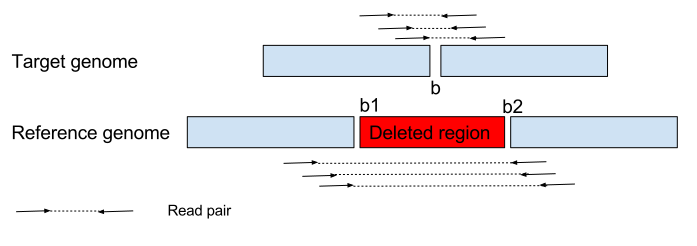
\includegraphics[width=\textwidth]{DeletionReadPairs}

Here reads around the breakpoint b will be mapped farther apart than expected on the reference
genome.

\paragraph{Lemma 2} Once again by definition of ARP, there is one read on each side of the breakpoint b, thus all reads in ARPs will be at most \verb|read_size + insert_size| away from the breakpoint, in the target genome.

Remembering properties 1 and 2, this tells us that we can have a boundary of fixed size in which
we can expect to catch all ARPs around a breakpoint.

\paragraph{Lemma 3} Respectively, should we have a group of ARPs supporting the same deletion we can say with a known confidence interval, that most ARPs to the left of the breakpoint b1 will be contained within \verb|insert_size + read_size| of the beginning of the leftmost supporting read. The same follows for the reads on the right of the breakpoint b2.

\subsubsection{Inversion} 

\begin{verbatim}
target: ->->->->->->->-> b1 <-<-<-<-<-<-<- b2 ->->->->->->->->
ref:    ->->->->->->->->    ->->->->->->->    ->->->->->->->->

where b1 and b2 are the two breakpoints
\end{verbatim}

Here ARPs are pairs where one read is in the inversed region and the other
is in the regular one (i.e. either one read left of b1 or one read right of b2). Indeed reads
between b1 and b2 will be mapped properly (because BWA is not sensitive to the order of the reads).

Reads in the inversed region will be mapped in the wrong direction, and farther away
than expected (as the region is inversed they will be moved closer to the other breakpoint).

We can see that if one read is left of b1, the other one will be mapped close to
b2 inside the inversed region and in the wrong direction, and that if one read is to the right
of b2, the other one will be mapped close to b1 in the inversed region and in the wrong direction
too.

We can also see by using properties 1 and 2, that reads outside the inversed region will be at most
\verb|insert_size + read_size| away from the breakpoints and that the same is true for reads inside
the inversed region.

\paragraph{Lemma 4} ARPs supporting an inversion will be distributed around the two
breakpoints within \verb|2*(insert_size + read_size)|.

\paragraph{Lemma 3} Respectively, should we have a group of ARPs supporting the same inversion we can say with a known confidence interval, that most ARPs around the left breakpoint will be contained within \verb|2 * (insert_size + read_size)| of the beginning of the leftmost supporting read. The same is trivially true for the right breakpoint.

\subsubsection{Tandem Duplication}

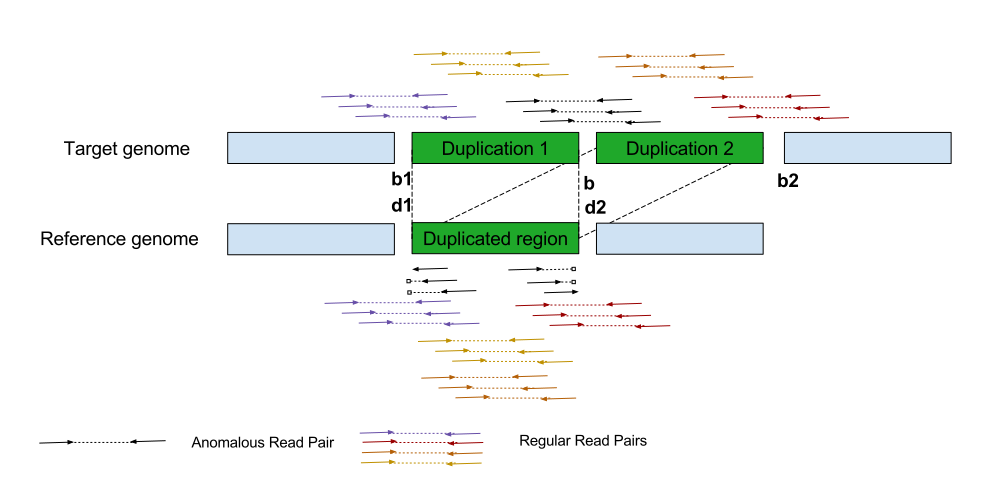
\includegraphics[width=\textwidth]{DuplicationReadPairs}

Here ARPs, are pairs that have one read on each side of breakpoint b, indeed
read pairs fully contained between b1 and b or b and b2, will be mapped properly on the
duplicated region.

\paragraph{Lemma 6} ARPs are aligned in the wrong direction (\verb|<- ->| instead of \verb|-> <-| for example), and inside the duplicated region, one within \verb|insert_size + read_size| to the right of d1, the other within \verb|insert_size + read_size| left of d2.
The read count in the duplicated region will be about the double of outside the duplicated region.

\paragraph{Lemma 7} It follows that should a region be duplicated more than once, the ARPs will be distributed the same way as with tandem duplication (except for higher read count and more ARPs).

\subsection{Conclusion}

\paragraph{Theorem 1} Putting all the lemmas together we can conclude that given a set of structural variants, there are two windows of size \verb|2 * (insert_size + read_size)| each, centered on the two breakpoints in the reference genome that contains most of the ARPs that will support it.

\paragraph{Theorem 2} Given a type of variant and a set of supporting ARPs, we can construct two windows of size \verb|2 * (insert_size + read_size)| that will contain the breakpoints in the reference genome.

\paragraph{Note} For tandem CNVs (and deletions) windows of size \verb|insert_size + read_size| would have sufficed to contain all the ARPs, however they would not have contained reads outside of the duplicated area (inside the deleted area), which would make us lose the RC information.
Taking larger windows also allows us to have a single window size for all our variants, and thus using the same model for all the variants.

\paragraph{Note} All the window sizes given here assumed that the reads and inserts were of the same size, when we know that they are variable, adding a few standards deviations will allow us to catch the read pairs with higher insert size or read size.

\end{document}